\section{Experimental Results}

% compare things against polling/triggered
% compare things against matchlist length / hashed Portals / multi-PTEs


We have gathered preliminary performance results using a prototype
implementation of \pdht running on the Portals reference
implementation~\cite{portals-code}.  Results were gathered on the Comet
system at the San Diego Supercomputer Center with access provided
through the Extreme Science and Engineering Discovery Environment (XSEDE)
program.  Comet contains nodes with several configurations; for our
experiments, we used the Intel\regtm Xeon\regtm E5 nodes.  There are 1944 such
nodes, which are constructed from Dell\othertm PowerEdge\othertm C6320 servers
containing dual 12-core Intel\regtm Xeon\regtm E5-2680 processors and 128
gigabytes of memory.  Nodes are connected using a Mellanox\othertm FDR 56 Gb/s
InfiniBand\othertm fabric.


\subsection{Experimental Setup}

To measure the effectiveness of implementing PDHT directly on top of Portals, 
we constructed an MPI version of PDHT. The MPI version provides a similar
functionality to PDHT and is implemented with a communication thread to 
manage insertion, access, and update requests. The MPI version relies
on the same hash function to determine rank and match bits, but
uses an efficient hash table on each local process~\cite{uthash} to
actually store the data elements. All tests are run using the MPICH
3.2 MPI run-time, configured to use a Portals 4 channel for all
communication operations.

\subsection{Communication Operation Costs}


As shown in Figure~\ref{fig:throughput}, we measure the weak scaling
of \pdht read operations on the key/value store by examining the
overall throughput of the system. Each process owns a fixed number of
hash table elements which are read by a neighboring process. The
system performs as expected under weak scaling, with overall system
throughput increasing with the number of processes involved. Of
particular interest, is the observation that throughput decreases as
the number of local hash table elements increases. Lower throughputs
with a larger number of elements imply higher overheads
within the message matching process in the Portals runtime.

To verify this, we measure the performance of retrieving elements from
the \pdht with respect to the number of elements on each process.
These results are shown in Figure~\ref{fig:mlen} and provide an
initial characterization of the lookup cost associated with our \pdht
implementation.  In contrast with traditional PGAS approaches,
building a remotely accessible key/value store on top of a mechanism
intended to support MPI message matching can add new overheads.  In
particular, the Portals message processing engine must traverse the
active match list until an ME that matches the given query is located.
In cases where the element does not exist, the Portals layer must
reach the end of the list to make this conclusion.  Thus, there is a
list traversal overhead that is proportional to the number of elements
visited before finding a match.

% latency with MPI vs. native

% throughput with MPI vs. native

% matchlist performance

% performance relative OpenSHMEM hash table implementation

% performance of MADNESS reconstruction MPI vs. native

% performance of MADNESS compression MPI vs. native

% performance of MADNESS diff MPI vs. native

% performance of sparse-matrix operation, MPI vs. native

\begin{figure}[ht]
  \center
  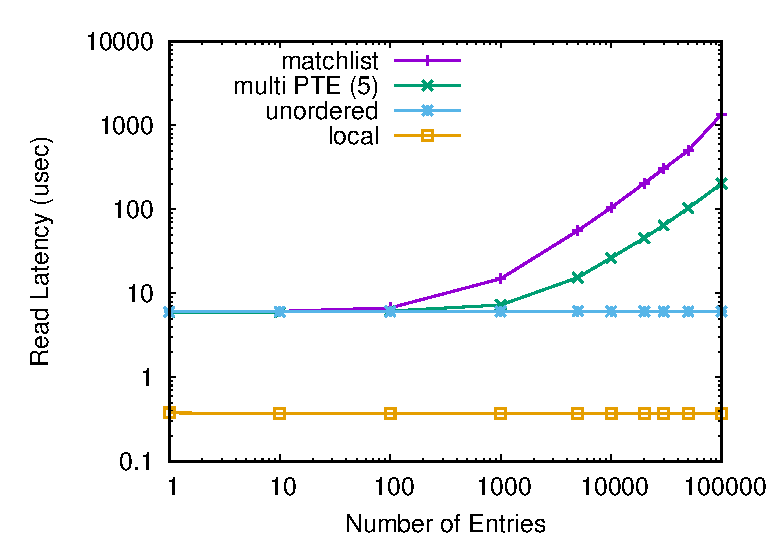
\includegraphics[width=.95\linewidth]{plots/pdhtlatency}
  \caption{PDHT Access Latencies ($\mu$sec)}
  \label{fig:6}
\end{figure}

\begin{figure}[ht]
  \center
  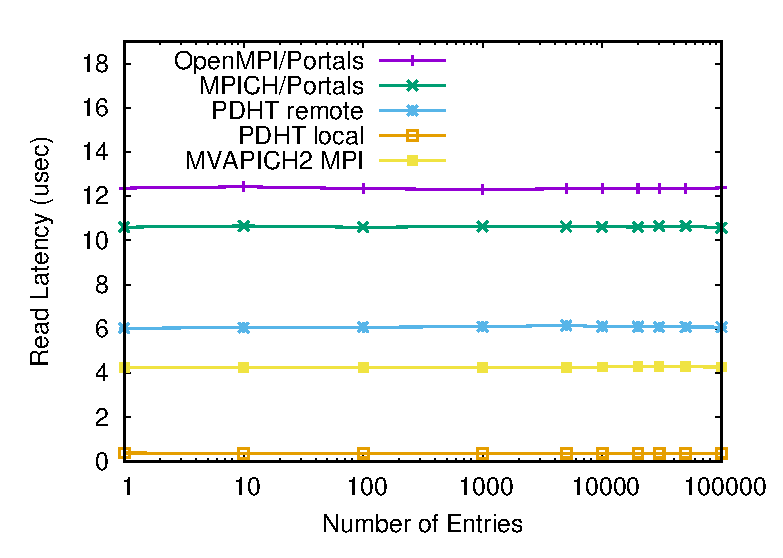
\includegraphics[width=.95\linewidth]{plots/mpilatency}
  \caption{PDHT and MPI Access Latency ($\mu$sec)}
  \label{fig:6}
\end{figure}

\begin{figure}
    \centering
    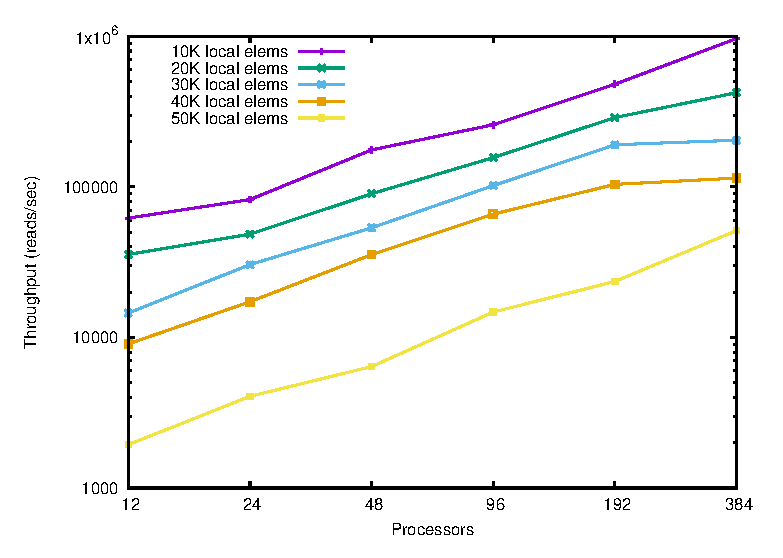
\includegraphics[width=.9\linewidth]{plots/throughput}
    %\caption{System throughput for a range of local volume (entries per node).}
    \caption{Aggregate system throughput for active list lengths of 10,000 to 50,000 local elements (8 byte elements).}
    \label{fig:throughput}
\end{figure}

\begin{figure}
    \centering
    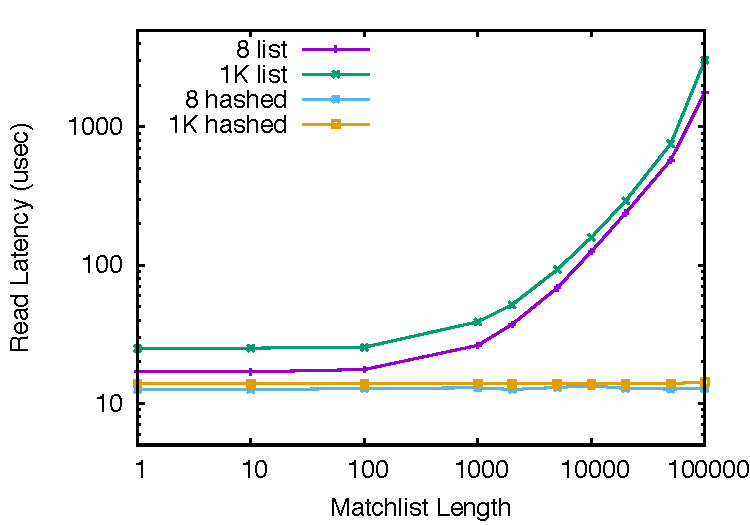
\includegraphics[width=.95\linewidth]{plots/mlen}
    %\caption{Read operation latency versus list depth for various size entries.}
    \caption{Latency for various size read operations measured over a range of active list (Portals match list) lengths. For this experiment, the expected matching depth of a list of length $L$ is $L/2$.}
    \label{fig:mlen}
\end{figure}

%\subsection{OpenSHMEM Benchmark}

\subsection{Sparse Matrix Multiplication}

This benchmark application computes the matrix product of two sparse 
matrices. Matrix sparsity is maintained by decomposing the source
matrices into tiles containing non-zero and zero elements. Tiles 
containing non-zero elements are added to the PDHT at the beginning of
the computation. The matrix multiplication then operates in a SPMD
fashion with each process requesting the necessary tiles to compute
the partial product. If either of the operand tiles are not in the
key/value store, the process continues on until it reaches a tile 
with non-zero elements. The performance of this benchmark is shown in
Figures~\ref{fig:4} and \ref{fig:5}.

\begin{figure}[ht]
  \center
  \fbox{\rule{2.5in}{0pt}\rule[-2.5in]{0pt}{4ex}}  
  \caption{Sparse-matrix multiplication weak scaling}
  \label{fig:4}
\end{figure}

\begin{figure}[ht]
  \center
  \fbox{\rule{2.5in}{0pt}\rule[-2.5in]{0pt}{4ex}}  
  \caption{Sparse-matrix multiplication strong scaling}
  \label{fig:5}
\end{figure}



\subsection{MADNESS}

The MADNESS quantum chemistry framework~\cite{thornton09} utilizes a
wavelet-based functions implemented using 3-6 dimensional spatial
representation trees. MADNESS trees represent functions with 
coefficients stored in either a scaling basis or a wavelet basis.
Certain operations on the function tree can only be performed in
one or the other basis modes. We consider three operations
provided by the MADNESS framework. The first two are conversion
operations: {\em compression}, in which scaling coefficients
are converted to the wavelet basis, and {\em reconstruction}, 
the complementary operation. The last operation is {\em differentiation},
in which the derivative of a function tree is computed with respect
to a single dimension. This operation requires coefficients 
to be present to the left and right of a node being differentiated,
which may cause compression or reconstruction operations to 
occur on neighboring subtrees. This is a highly irregular operation
and is easily expressed using spatial tree coordinates, but is
very difficult using traditional message-passing (due to tree
irregularity) and PGAS (due to physical addressing requirements).

Figures~\ref{fig:1}--\ref{fig:3} show the performance of the
Portals-based PDHT implementation relative to the MPI implementation.

\begin{figure}[ht]
  \center
  \fbox{\rule{2.5in}{0pt}\rule[-2.5in]{0pt}{4ex}}  
  \caption{MADNESS compression performance ($\mu$ sec)}
  \label{fig:1}
\end{figure}

\begin{figure}[ht]
  \center
  \fbox{\rule{2.5in}{0pt}\rule[-2.5in]{0pt}{4ex}}  
  \caption{MADNESS reconstruction performance ($\mu$ sec)}
  \label{fig:2}
\end{figure}

\begin{figure}[ht]
  \center
  \fbox{\rule{2.5in}{0pt}\rule[-2.5in]{0pt}{4ex}}  
  \caption{MADNESS differentiation performance ($\mu$ sec)}
  \label{fig:3}
\end{figure}


%%% Local Variables:
%%% mode: latex
%%% TeX-master: "paper"
%%% End:
